% ============================================================
\chapter{\'Equation de la Chaleur}
\label{ch:chaleur}
% ============================================================

C'est pour comprendre la propagation de la chaleur que Joseph Fourier a d\'evelopp\'e les s\'eries qui portent son nom. Son \emph{Th\'eorie analytique de la chaleur} (1822) est l'un des textes fondateurs de la physique math\'ematique. L'\'equation de la chaleur --- la plus simple des EDP paraboliques --- d\'ecrit un ph\'enom\`ene irr\'eversible~: un profil de temp\'erature initial se lisse au fil du temps, les pics s'aplatissent, les gradients s'estompent. Contrairement \`a l'\'equation d'onde, l'information se propage \`a vitesse infinie, et contrairement \`a l'\'equation de transport, les solutions deviennent imm\'ediatement r\'eguli\`eres. Ces propri\'et\'es, surprenantes et contre-intuitives, font de l'\'equation de la chaleur le prototype de toutes les \'equations de diffusion.

\section{Motivation physique et formulation}

L'\'equation de la chaleur d\'ecrit la diffusion thermique dans un milieu
conducteur. Si $u(x,t)$ repr\'esente la temp\'erature, la loi de Fourier
($\vec{q} = -k\nabla u$) combin\'ee \`a la conservation de l'\'energie donne~:

\begin{definition}[\'Equation de la chaleur]
L'\textbf{\'equation de la chaleur} en dimension $n$ est~:
\begin{equation}\label{eq:chaleur}
    u_t - \kappa\, \Delta u = f(x,t), \quad x \in \Omega \subset \R^n,\; t > 0,
\end{equation}
o\`u $\kappa > 0$ est la diffusivit\'e thermique. Le cas $f = 0$ est dit
\textbf{homog\`ene}.
\end{definition}

\begin{intuition}
L'\'equation de la chaleur lisse les irr\'egularit\'es~: m\^eme si la
temp\'erature initiale est discontinue, la solution devient instantan\'ement
$C^\infty$ pour $t > 0$. C'est l'\textbf{effet r\'egularisant} de la diffusion.
Cependant, l'information se propage \`a vitesse infinie (pas de front d'onde).
\end{intuition}

\section{Solution fondamentale}

\begin{definition}[Noyau de la chaleur]
Le \textbf{noyau de la chaleur} (ou solution fondamentale) en dimension $n$ est~:
\begin{equation}\label{eq:noyau_chaleur}
    \Phi(x,t) = \frac{1}{(4\pi\kappa t)^{n/2}}
    \exp\!\left(-\frac{\abs{x}^2}{4\kappa t}\right), \quad t > 0.
\end{equation}
\end{definition}

\begin{theoreme}[Propri\'et\'es du noyau de la chaleur]
Le noyau $\Phi$ v\'erifie~:
\begin{enumerate}
    \item $\Phi_t = \kappa\, \Delta \Phi$ pour $t > 0$, $x \neq 0$.
    \item $\Phi(x,t) > 0$ pour tout $x \in \R^n$, $t > 0$.
    \item $\int_{\R^n} \Phi(x,t)\, dx = 1$ pour tout $t > 0$.
    \item $\Phi(\cdot, t) \to \delta_0$ au sens des distributions quand $t \to 0^+$.
\end{enumerate}
\end{theoreme}

\begin{proof}
(1) V\'erification directe en dimension $n = 1$. On a
$\Phi(x,t) = (4\pi\kappa t)^{-1/2} e^{-x^2/(4\kappa t)}$. Calculons~:
\[
    \Phi_t = \Phi\left(-\frac{1}{2t} + \frac{x^2}{4\kappa t^2}\right),
    \quad
    \Phi_x = -\frac{x}{2\kappa t}\Phi, \quad
    \Phi_{xx} = \left(\frac{x^2}{4\kappa^2 t^2} - \frac{1}{2\kappa t}\right)\Phi.
\]
Donc $\Phi_t = \kappa\, \Phi_{xx}$.

(3) Par le changement $y = x/\sqrt{4\kappa t}$~:
$\int_{\R^n} \Phi\, dx = \pi^{-n/2}\int_{\R^n} e^{-\abs{y}^2}\, dy = 1$.
\end{proof}

\begin{center}
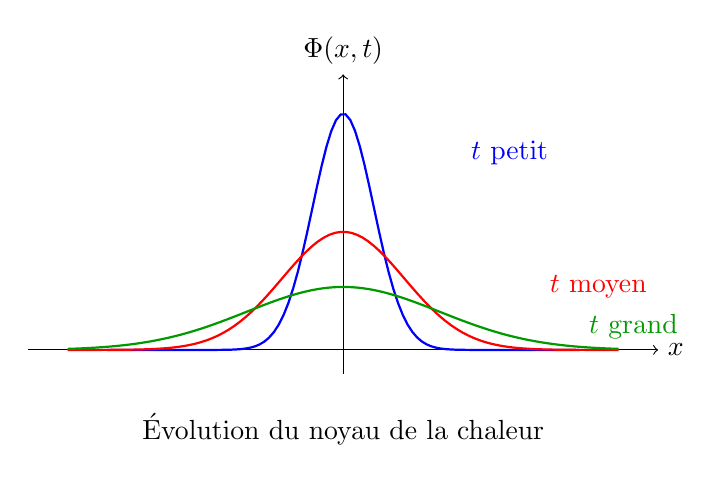
\begin{tikzpicture}[scale=1.0]
    \draw[->] (-4,0) -- (4,0) node[right] {$x$};
    \draw[->] (0,-0.3) -- (0,3.5) node[above] {$\Phi(x,t)$};
    % t petit
    \draw[thick, blue, domain=-3:3, samples=100]
        plot (\x, {3*exp(-\x*\x/0.3)});
    \node[blue, right] at (1.5, 2.5) {$t$ petit};
    % t moyen
    \draw[thick, red, domain=-3.5:3.5, samples=100]
        plot (\x, {1.5*exp(-\x*\x/1.2)});
    \node[red, right] at (2.5, 0.8) {$t$ moyen};
    % t grand
    \draw[thick, green!60!black, domain=-3.5:3.5, samples=100]
        plot (\x, {0.8*exp(-\x*\x/3)});
    \node[green!60!black, right] at (3, 0.3) {$t$ grand};
    \node at (0, -1) {\'Evolution du noyau de la chaleur};
\end{tikzpicture}
\end{center}

\section{Probl\`eme de Cauchy sur $\R^n$}

\begin{theoreme}[Solution par convolution]
Si $u_0 \in L^\infty(\R^n) \cap C(\R^n)$, la solution du probl\`eme de Cauchy~:
\[
    u_t = \kappa\, \Delta u, \quad u(x,0) = u_0(x),
\]
est donn\'ee par la convolution~:
\begin{equation}\label{eq:solution_cauchy_chaleur}
    u(x,t) = (\Phi(\cdot, t) * u_0)(x)
    = \int_{\R^n} \Phi(x-y, t)\, u_0(y)\, dy.
\end{equation}
De plus, $u \in C^\infty(\R^n \times (0,\infty))$.
\end{theoreme}

\begin{proof}[Id\'ee de la preuve]
On peut d\'eriver sous le signe int\'egral car $\Phi$ est $C^\infty$ pour
$t > 0$ et d\'ecro\^it exponentiellement. La condition initiale d\'ecoule
de la propri\'et\'e (4) du noyau~: $\Phi(\cdot, t) * u_0 \to u_0$
quand $t \to 0^+$.
\end{proof}

\begin{formules}[title=\textbf{\'Equation de la chaleur --- formules cl\'es}]
\begin{itemize}
    \item Noyau ($n=1$)~: $\Phi(x,t) = \frac{1}{\sqrt{4\pi\kappa t}}\, e^{-x^2/(4\kappa t)}$.
    \item Solution de Cauchy~: $u = \Phi * u_0$.
    \item Avec source~: $u = \Phi * u_0 + \int_0^t \Phi(\cdot, t-s) * f(\cdot, s)\, ds$
          (formule de Duhamel).
\end{itemize}
\end{formules}

\section{Principe du maximum pour l'\'equation de la chaleur}

\begin{theoreme}[Principe du maximum faible]
Soit $\Omega \subset \R^n$ un ouvert born\'e et
$\Omega_T = \Omega \times (0,T]$. Si $u \in C^{2,1}(\Omega_T) \cap C(\overline{\Omega_T})$
satisfait $u_t - \kappa\Delta u \leq 0$ dans $\Omega_T$, alors~:
\begin{equation}\label{eq:max_faible_chaleur}
    \max_{\overline{\Omega_T}} u = \max_{\Gamma_T} u,
\end{equation}
o\`u $\Gamma_T = (\overline{\Omega} \times \{0\}) \cup (\partial\Omega \times [0,T])$
est la \textbf{fronti\`ere parabolique}.
\end{theoreme}

\begin{proof}
Supposons par l'absurde que le maximum est atteint en un point int\'erieur
$(x_0, t_0) \in \Omega_T$ avec $t_0 > 0$. Alors $\nabla u(x_0, t_0) = 0$,
$D^2 u(x_0, t_0) \leq 0$ (semi-d\'efinie n\'egative), donc
$\Delta u(x_0, t_0) \leq 0$. De plus, $u_t(x_0, t_0) \geq 0$ (car le
maximum est atteint \`a $t_0$). Donc
$u_t - \kappa\Delta u \geq 0$ en $(x_0, t_0)$, contradiction avec
$u_t - \kappa\Delta u \leq 0$ (sauf si \'egalit\'e). On conclut par
perturbation en consid\'erant $v = u - \varepsilon t$.
\end{proof}

\begin{center}
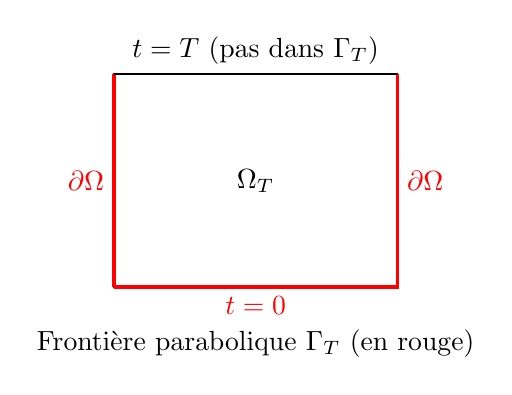
\begin{tikzpicture}[scale=0.9]
    \draw[thick] (0,0) rectangle (4,3);
    % Frontière parabolique en rouge
    \draw[very thick, red] (0,0) -- (4,0) -- (4,3);
    \draw[very thick, red] (0,0) -- (0,3);
    \draw[very thick, red] (0,0) -- (4,0);
    % Labels
    \node at (2, 1.5) {$\Omega_T$};
    \node[red, below] at (2, 0) {$t = 0$};
    \node[red, left] at (0, 1.5) {$\partial\Omega$};
    \node[red, right] at (4, 1.5) {$\partial\Omega$};
    \draw[dashed] (0,3) -- (4,3);
    \node[above] at (2,3) {$t = T$ (pas dans $\Gamma_T$)};
    \node at (2, -0.8) {Fronti\`ere parabolique $\Gamma_T$ (en rouge)};
\end{tikzpicture}
\end{center}

\begin{corollaire}[Unicit\'e]
Le probl\`eme de Cauchy-Dirichlet pour l'\'equation de la chaleur
(sur un domaine born\'e) admet au plus une solution classique.
\end{corollaire}

\begin{proof}
Si $u$ et $v$ sont deux solutions, $w = u - v$ satisfait $w_t = \kappa\Delta w$
avec $w = 0$ sur $\Gamma_T$. Par le principe du maximum, $w \leq 0$ dans
$\overline{\Omega_T}$. En appliquant le m\^eme argument \`a $-w$, on obtient
$w \geq 0$, donc $w = 0$.
\end{proof}

\section{R\'egularit\'e et effet lissant}

\begin{theoreme}[R\'egularit\'e infinie]
Si $u$ est solution de $u_t = \kappa\Delta u$ dans $\Omega_T$ avec
$u_0 \in L^2(\Omega)$, alors $u \in C^\infty(\Omega \times (0,T])$.
\end{theoreme}

\begin{attention}[title=\textbf{Irr\'eversibilit\'e}]
L'\'equation de la chaleur est irr\'eversible en temps~: on ne peut pas,
en g\'en\'eral, remonter le temps. Le probl\`eme $u_t = -\kappa\Delta u$
avec donn\'ee finale est mal pos\'e au sens de Hadamard.
\end{attention}

\section{Comportement asymptotique}

\begin{theoreme}[D\'ecroissance en temps]
Soit $u$ la solution de $u_t = \kappa\Delta u$ sur $\R^n$ avec
$u_0 \in L^1(\R^n) \cap L^\infty(\R^n)$. Alors~:
\begin{enumerate}
    \item $\norm{u(\cdot,t)}_{L^\infty} \leq \frac{C}{t^{n/2}}\norm{u_0}_{L^1}$.
    \item $\norm{u(\cdot,t)}_{L^2}$ est d\'ecroissante en $t$.
    \item $\int_{\R^n} u(x,t)\, dx = \int_{\R^n} u_0(x)\, dx$ (conservation de la masse).
\end{enumerate}
\end{theoreme}

\begin{proof}
(2) Calculons~:
\[
    \frac{d}{dt}\frac{1}{2}\int_{\R^n} u^2\, dx
    = \int_{\R^n} u\, u_t\, dx
    = \kappa\int_{\R^n} u\, \Delta u\, dx
    = -\kappa\int_{\R^n} \abs{\nabla u}^2\, dx \leq 0.
\]
(3) En int\'egrant l'\'equation et utilisant le th\'eor\`eme de la divergence~:
$\frac{d}{dt}\int u\, dx = \kappa\int \Delta u\, dx = 0$ (si $u$ d\'ecro\^it
suffisamment \`a l'infini).
\end{proof}

\section{Formule de Duhamel}

\begin{theoreme}[Principe de Duhamel]
La solution du probl\`eme non homog\`ene~:
\[
    u_t - \kappa\Delta u = f(x,t), \quad u(x,0) = u_0(x),
\]
sur $\R^n$ est~:
\begin{equation}\label{eq:duhamel}
    u(x,t) = \int_{\R^n} \Phi(x-y,t)\, u_0(y)\, dy
    + \int_0^t \int_{\R^n} \Phi(x-y, t-s)\, f(y,s)\, dy\, ds.
\end{equation}
\end{theoreme}

\begin{intuition}
Le principe de Duhamel est l'analogue pour les EDP de la m\'ethode de
variation des constantes pour les EDO. Le terme source $f$ est trait\'e
comme une superposition continue de conditions initiales appliqu\'ees
\`a chaque instant $s$.
\end{intuition}

\section{\'Equation de la chaleur sur un intervalle born\'e}

\begin{exemple}
R\'esoudre compl\`etement~:
\[
    \begin{cases}
        u_t = u_{xx}, & 0 < x < \pi,\; t > 0,\\
        u(0,t) = u(\pi,t) = 0,\\
        u(x,0) = x(\pi - x).
    \end{cases}
\]
Par s\'eparation des variables (cf.\ Chapitre~\ref{ch:fourier}), les modes
propres sont $X_n = \sin(nx)$, $\lambda_n = n^2$, et~:
\[
    u(x,t) = \sum_{n=1}^{\infty} b_n \sin(nx)\, e^{-n^2 t}.
\]
Les coefficients de Fourier en sinus de $f(x) = x(\pi-x)$ sont~:
\[
    b_n = \frac{2}{\pi}\int_0^\pi x(\pi-x)\sin(nx)\, dx
    = \begin{cases} \frac{8}{n^3\pi} & \text{si $n$ impair,}\\ 0 & \text{si $n$ pair.}\end{cases}
\]
Donc~:
\[
    u(x,t) = \frac{8}{\pi}\sum_{k=0}^{\infty}
    \frac{\sin((2k+1)x)}{(2k+1)^3}\, e^{-(2k+1)^2 t}.
\]
Pour $t$ grand, $u(x,t) \approx \frac{8}{\pi}\sin(x)\, e^{-t}$~:
seul le premier mode survit.
\end{exemple}

\section{Conditions aux limites non homog\`enes}

Pour traiter $u(0,t) = g_0(t)$, $u(L,t) = g_1(t)$, on pose
$v(x,t) = u(x,t) - w(x,t)$ o\`u $w$ est un \textbf{rel\`evement} des
conditions aux limites~:
\[
    w(x,t) = g_0(t) + \frac{x}{L}\bigl(g_1(t) - g_0(t)\bigr).
\]
Alors $v$ satisfait l'\'equation de la chaleur avec conditions homog\`enes
et un terme source modifi\'e.

\section{Exercices}

\begin{exercice}
V\'erifier que $\Phi(x,t) = \frac{1}{\sqrt{4\pi\kappa t}}\, e^{-x^2/(4\kappa t)}$
satisfait $\Phi_t = \kappa\, \Phi_{xx}$ pour $t > 0$.
\end{exercice}

\begin{exercice}
R\'esoudre $u_t = u_{xx}$ sur $\R$ avec $u(x,0) = e^{-\abs{x}}$.
\end{exercice}

\begin{exercice}
Montrer que l'\'energie $E(t) = \frac{1}{2}\int_0^L u^2(x,t)\, dx$
est d\'ecroissante pour l'\'equation de la chaleur avec conditions de
Dirichlet homog\`enes. Quelle est la vitesse de d\'ecroissance~?
\end{exercice}

\begin{exercice}
R\'esoudre $u_t = u_{xx} + \sin(x)$ sur $(0,\pi)$ avec $u(0,t) = u(\pi,t) = 0$
et $u(x,0) = 0$. \emph{Indication~:} chercher une solution stationnaire
puis utiliser Duhamel.
\end{exercice}

\begin{exercice}
Soit $u$ solution de $u_t = u_{xx}$ sur $(0,1)$ avec $u(0,t) = 0$,
$u(1,t) = 1$, $u(x,0) = x$. Trouver la solution stationnaire et montrer
que $u$ converge vers celle-ci.
\end{exercice}

\begin{exercice}[Autosimilarit\'e]
Chercher une solution de $u_t = u_{xx}$ sous la forme
$u(x,t) = t^{-\alpha} f(\xi)$ avec $\xi = x/\sqrt{t}$.
D\'eterminer $\alpha$ et l'EDO v\'erifi\'ee par $f$.
\end{exercice}

\begin{exercice}
Montrer que la temp\'erature maximale d\'ecro\^it au cours du temps pour
l'\'equation de la chaleur sur un domaine born\'e avec conditions de
Dirichlet homog\`enes. \emph{Indication~:} utiliser le principe du maximum.
\end{exercice}
